\section{Budget}


\subsection{Revenue}
We have compared the predicted and actual revenues from previous reports and used these to estimate our expected revenue. To maintain reasonable accuracy in the budget, we were financially conservative in our estimates to account for fluctuating economy and attendance numbers. Should our bid be selected, these conservative estimates will result in a smoother planning and execution process. We have also accounted an estimated number of waived professional registration based on previous conferences. This  correlates to the number of waived fees given in our expected tier sponsorship figures and also factors in discounts to speakers, panelists, and workshop instructors. \\

\begin{table}[H]
\centering
\caption*{\textbf{Attendance}}
\begin{tabular}{|c|c|c|c|}
\hline
    \textbf{Item} & \textbf{Quantity} & \textbf{Cost} & \textbf{Subtotal}	\\ 
\hline
	Student			&	443	&	\$40	&	\$17,720						\\
	Professional	&	127	& 	\$250	&	\$31,750						\\
	Waived			&	60	& 	-\$250	&	-\$15,000						\\
\hline
	\multicolumn{3}{|r|}{\textbf{Attendance Total:}}	&	\$34,470		\\
\hline
\end{tabular}
\end{table}

\vspace{10mm}

\begin{table}[H]
\centering
\caption*{\textbf{Sponsors}}
\begin{tabular}{|c|c|c|c|}
\hline
    \textbf{Package} & \textbf{Quantity} & \textbf{Cost} & \textbf{Subtotal}	\\ 
\hline
	World Savior	&	1	&	\$30,000	&	\$30,000						\\
	National Hero	&	3	& 	\$15,000	&	\$45,000						\\
	Local Prodigy	&	5	& 	\$10,000	&	\$50,000						\\
	Lifesaver		&	6	& 	\$5,000		&	\$30,000						\\
	Exhibitor+		&	3	& 	\$3,500		&	\$10,500						\\
	Exhibitor		&	5	& 	\$2,500		&	\$12,500						\\
	Good Samaritan	&	10	& 	\$1,500		&	\$15,000						\\
	Contributor		&	8	& 	\$1,000		&	\$8,000							\\
\hline
	\multicolumn{3}{|r|}{\textbf{Sponsors Total:}}	&	\$201,000				\\
\hline
\end{tabular}
\end{table}

\vspace{10mm}

\begin{table}[H]
\centering
\begin{tabular}{|c|}
\hline
    \textbf{Total Revenue: \$235,470}\\ 
\hline
\end{tabular}
\end{table}

\subsection{Expenses}

\subsection{Sponsorship and Fundraising}
The sponsorship breakdown for our conference pulls from averages of sponsorship packages in the last several conferences, with for main tiers that tie into the conference theme for the largest representation in the conference and visibility in the career fair, socials, sessions, technical, and meals as well as in conference shirts and attendee bags. Using two tiers for an exhibitor package allows for a platform for DOE national laboratories to participate, with the higher tier having logo representation on shirts as well as the opportunity to sponsor a coffee break or lunch \& learn session. Lastly, two packages are left to benefactors who are recognized in the conference program and represent the anticipated support from ANS divisions or local industry or University of Illinois contributors (or some generous contributions from out-of-state companies!). 

\begin{figure}[H]
	\centering
	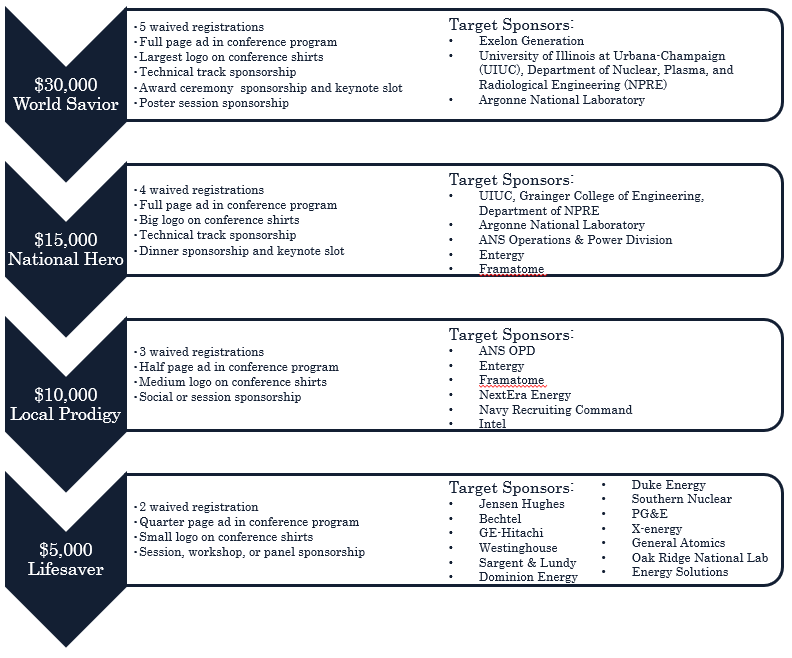
\includegraphics[width=0.75\textwidth]{sponsors1.png}	
\end{figure} 

\begin{figure}[H]
	\centering
	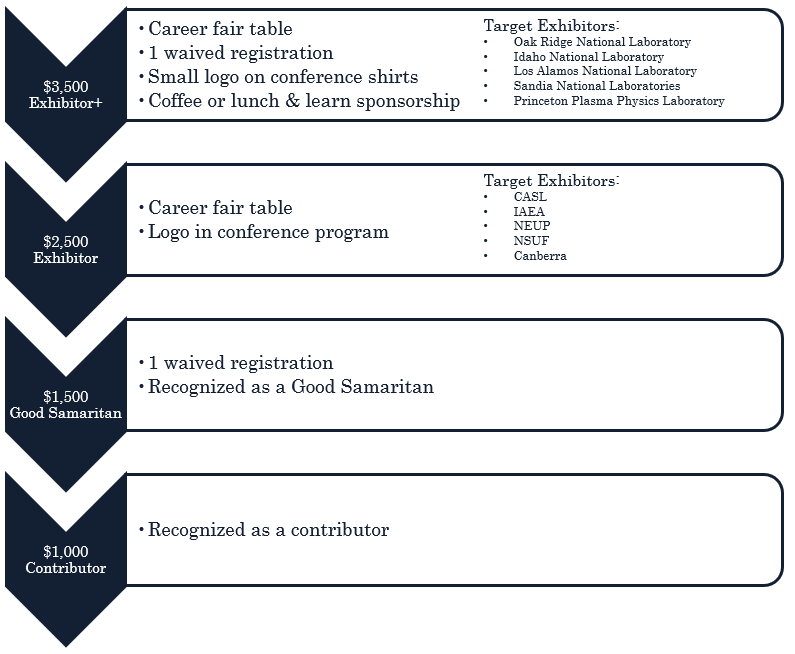
\includegraphics[width=0.75\textwidth]{sponsors2.png}	
\end{figure} 

\subsection{Banking}

In order to properly handle all of the conference expenses, two accounts will be used. One account will be with the national ANS headquarters, and the second will be a local checking account through Busey Bank. Our student section currently holds a checking account with Busey Bank and has developed a working relationship with them. Similar to previous conferences, the national ANS account will be the primary account due to their previous experience in handling conference funds and their 501(c)(3) tax exemption status. Although an account with the national ANS organization is currently not maintained by the UIUC local chapter, should this bid be selected, the opening of an account would happen almost immediately. An established local checking account with Busey Bank allows for convenience when using them as a secondary account. The student section account has been maintained for a number of years, allowing for adequate knowledge of Busey’s policies and a stable relationship to be established with the local branch. A new account would be opened, such that the student chapter funds and the conference funds are completely separate and require different oversight. This account will be used for small expenses that can occur during the conference. Although the ANS-managed account could be used for such purposes, the presence of a local branch allows for more flexibility if a purchase becomes time sensitive. Should the additional Busey Bank account be unobtainable, an account would be established with Chase instead. If ANS National desires to manage all funds, accommodations will be made to consolidate the funds.

\subsubsection{Financial Oversight}
Financial integrity must be maintained when providing a conference of this size. To do so, diligent oversight will be practiced for all transactions related to the conference. Expense requests will be required for all transactions. These requests must carefully outline the reason for the purchase and the total cost. If the purchase is reoccuring, automation will be required at the time of request. These requests will require the approval of both conference chairs in addition to the financial director. Only the conference chairs and the financial director will have authority, assuming the previously mentioned permission, to complete transactions on the Busey Bank account. To ensure transparency, the financial director will update a public record containing all transactions. 

\subsection{Financial Contingency}

\subsection{Cost of Attendance and Student Reimbursement}
The cost of attending the student conference, per student, varies among schools and is highly dependent on distance from UIUC and the preferred mode of travel. We will assume that minimizing cost is a priority for schools, thus number of persons per hotel room is double the number of beds. 